\chapter{Initial Data Analysis}\label{Sec:Initial Data Analysis}

A brief characterization of the data employed in this evaluation is given. 

In order to diagnose to what extent an algorithm suffers from , it will be useful to have another dataset.
The da, that is understanding what properties of the data differ between GBS and GESIS. 

For completeness, we provide a description of the feature engineering process. We specify the list of transformations that are sequentially applied to each group of features in order to prepare the input for the final model. All
missing values are imputed based on domain-expert decisions. Outliers are handledmanually. Wesplittheinputdataintothreegroupsoffeatures: continuous, categorical and text.

\begin{figure}[ht]
	\begin{center}
		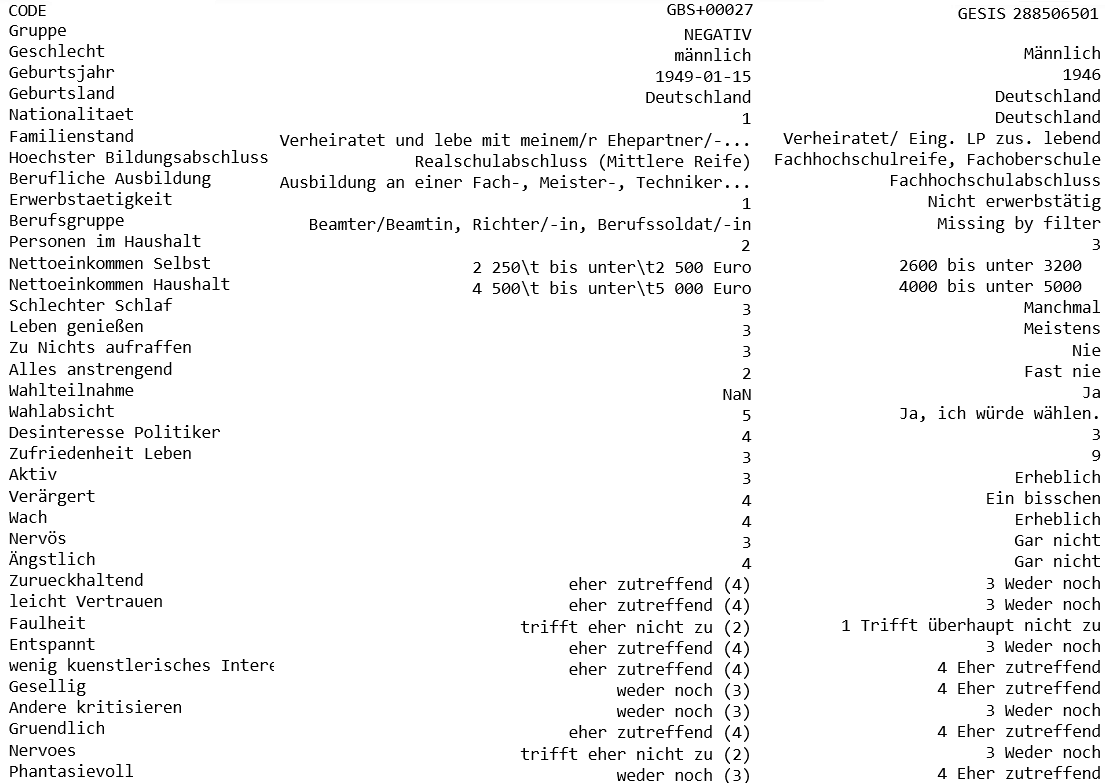
\includegraphics[scale=0.53,angle=0]{fig/values_compare}
		\label{std}
		\caption{GBS - GESIS attribute and value comparison. Not all attributes are used in every learning task. See GitHub documentation for more information.}
	\end{center}
\end{figure}

Continuous Features First of all, we perform logarithmic transformation of the skewed continuous features in order to reduce the skewness. Second, westandardizethecontinuousfeaturesbyremovingth emeanandscalingto unit variance. Centering and scaling happen independently on each feature by computing the relevant statistics on the samples in the dataset.
Categorical Features We encode all categorical variables with values between 0 and nclasses-1 where nclasses is the number of distinct categorical values for a given variable. Next, we perform one-hot encoding.

This combination of class imbalance with non-stationary environments poses significant and interesting practical problems for classification

\begin{figure}[ht]
	\begin{center}
		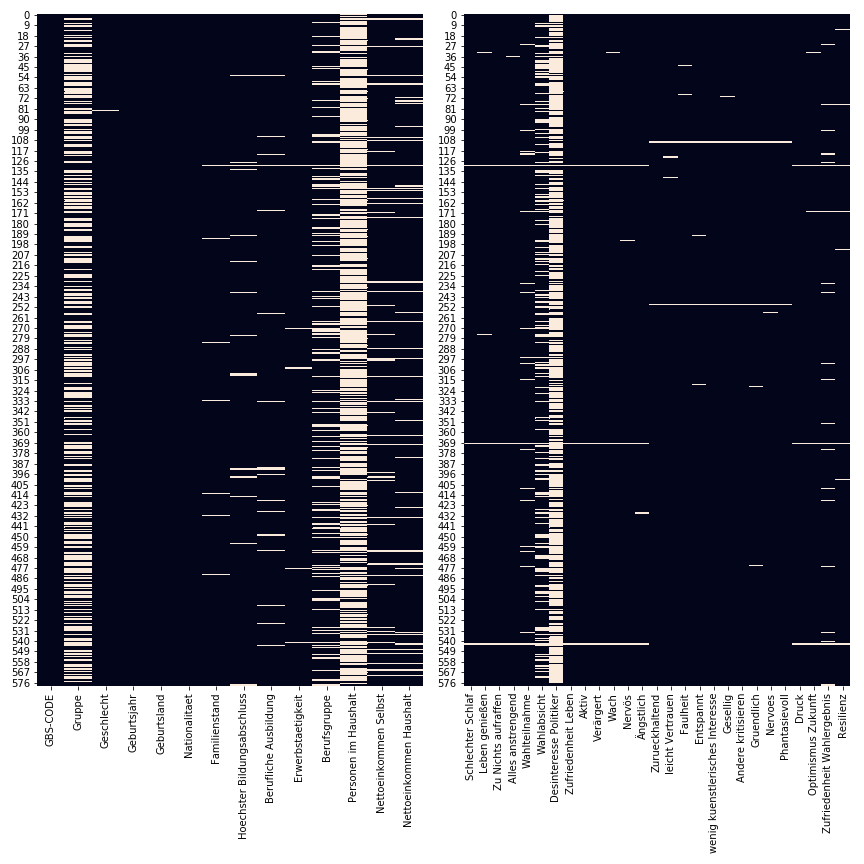
\includegraphics[scale=0.50,angle=0]{fig/gbs_missing}
		\label{std}
		\caption{GBS missing value comparison.}
	\end{center}
\end{figure}

\begin{figure}[ht]
	\begin{center}
		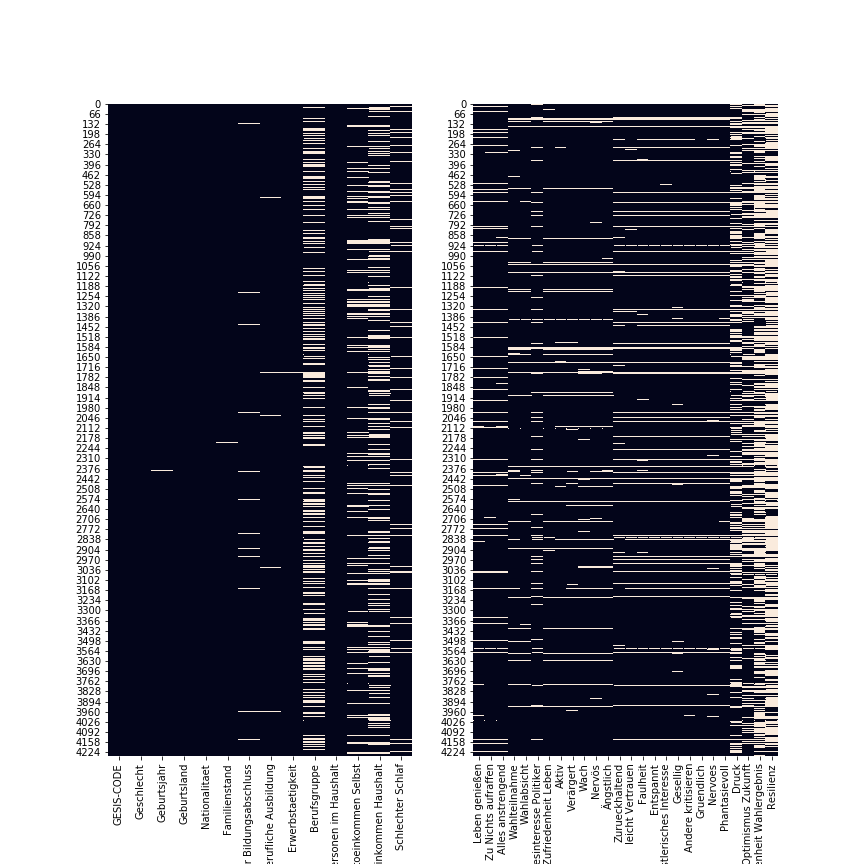
\includegraphics[scale=0.50,angle=0]{fig/gesis_missing}
		\label{std}
		\caption{GESIS missing value comparison.}
	\end{center}
\end{figure}

\section{Political Participation and Resilience}

\begin{figure}[ht]
	\begin{center}
		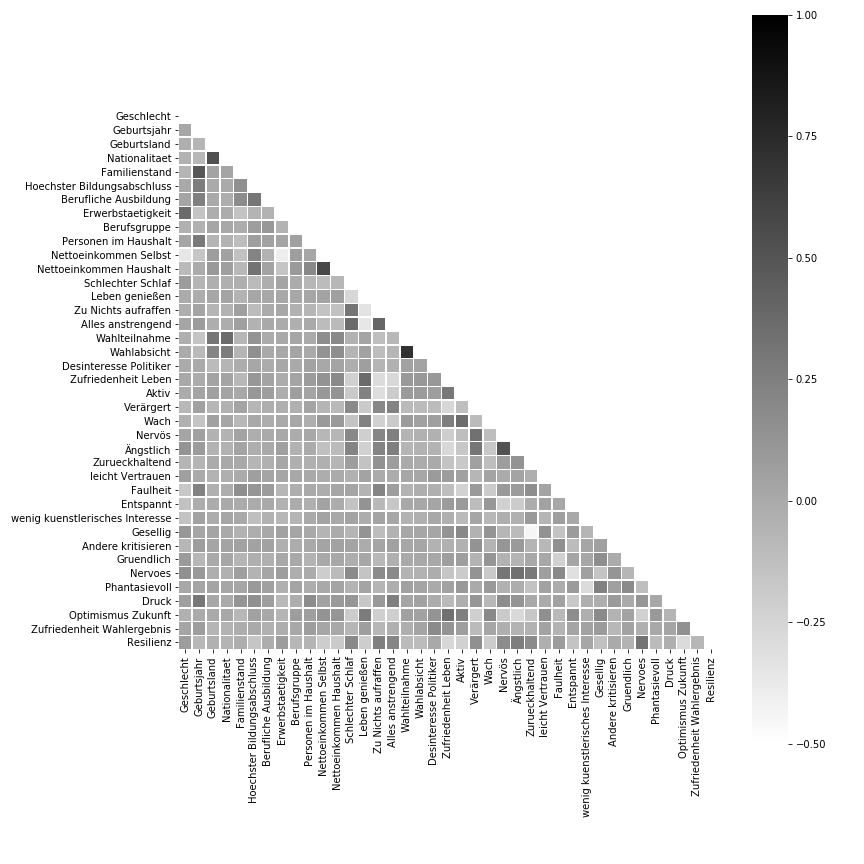
\includegraphics[scale=0.52,angle=0]{fig/gesis_corr}
		\label{std}
		\caption{GBS - GESIS attribute and value comparison.}
	\end{center}
\end{figure}

\begin{figure}[ht]
	\begin{center}
		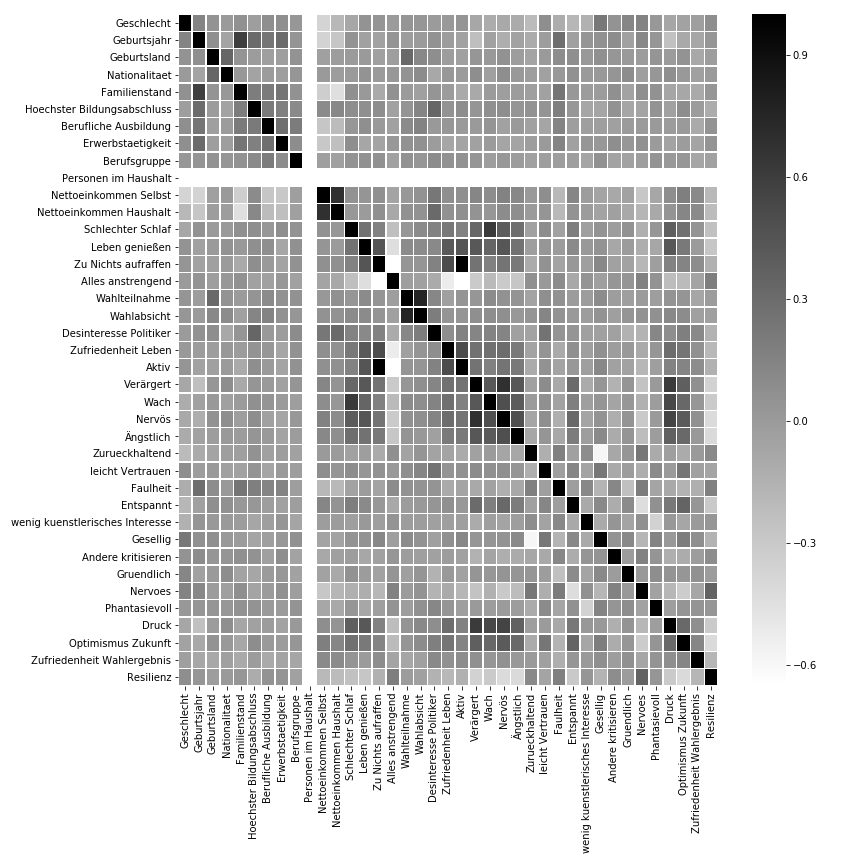
\includegraphics[scale=0.52,angle=0]{fig/gbs_corr}
		\label{std}
		\caption{GBS - GESIS attribute and value comparison.}
	\end{center}
\end{figure}

\subsection{The Big Five Dimensions}

\begin{figure}[ht]
	\begin{center}
		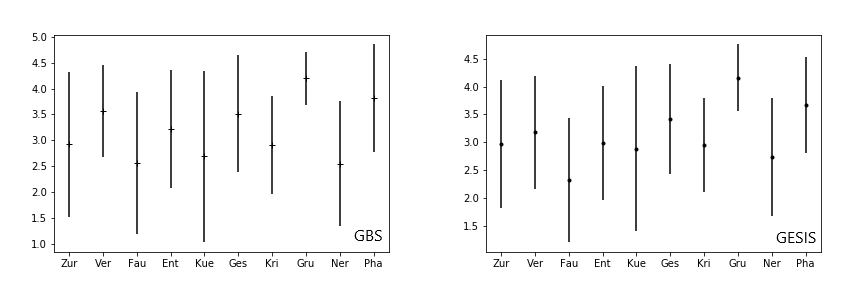
\includegraphics[scale=0.55,angle=0]{fig/std_figure}
		\label{std}
		\caption{Mean and standard deviation of BFI-10 Items:\textit{"A Short Scale for Assessing the Big Five Dimensions of Personality"}.}
	\end{center}
\end{figure}

The Big Five is an empirically-derived model of human personality and psyche. When factor analysis is applied to personality survey data, five clusters of traits consistently emerge. The BFI-10 is a 10-item scale measuring the Big Five personality traits, two BFI items for each dimension, representing both the high and low pole of each factor [Fig X]. Likert scales are the most frequently used instruments in GBS and GESIS. They consist of statements which measure the intensity of one's estimation towards the preceding statement. Respondents are asked to rate the BFI-10 items on a level of agreement on a consistent rating scale ranging from "Strongly Agree (5)" to Strongly Disagree (1)" for all items in both survey.

\begin{figure}[ht]
	\begin{center}
		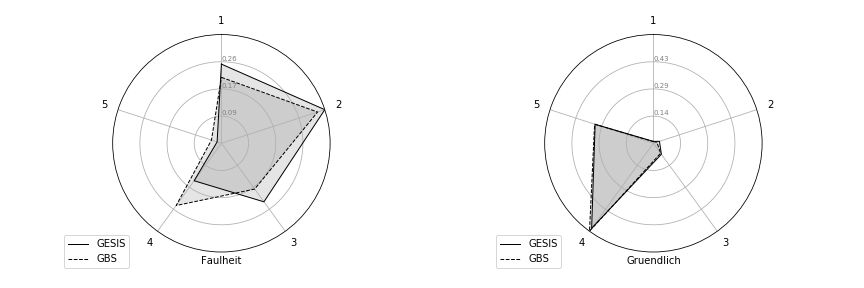
\includegraphics[scale=0.55,angle=0]{fig/Conscientiousness_figure}
		\label{Conscientiousness}
		\caption{Conscientiousness: the degree of organization, self-regulation, and responsibility one exhibits. \textit{"I see myself as someone who tends to be lazy."}(left). \textit{"I see myself as someone who does a thorough job."}(right).}
	\end{center}
\end{figure}

                \begin{figure}[ht]
                \begin{center}
                   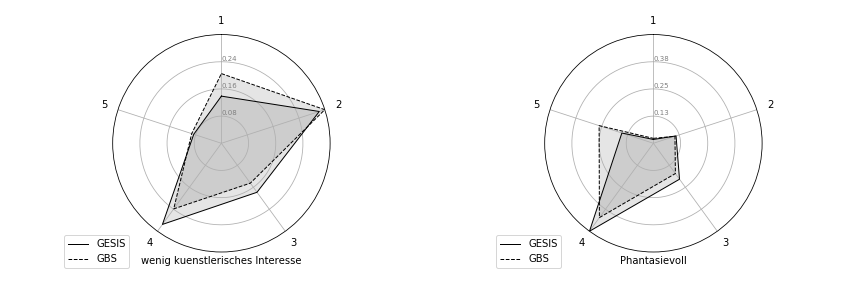
\includegraphics[scale=0.55,angle=0]{fig/Opennessfigure}
	         \label{Openness}
	         \caption{ Openness: \textit{" I see myself as someone who has few artistic interests"}(left). \textit{"I see myself as someone who has an active imagination"}(right).}
                \end{center}
                \end{figure}

                \begin{figure}[ht]
                \begin{center}
                   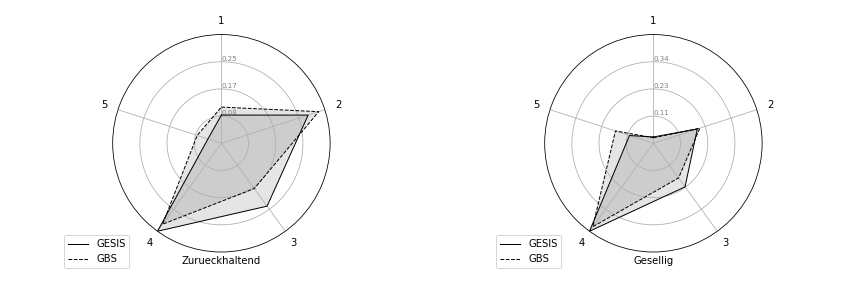
\includegraphics[scale=0.55,angle=0]{fig/Extraversionfigure}
	         \label{Extraversion}
	         \caption{Extraversion: \textit{"I see myself as someone who is reserved."}(left). \textit{"I see myself as someone who is outgoing, sociable. "}(right).}
                \end{center}
                \end{figure}

                \begin{figure}[ht]
                \begin{center}
                   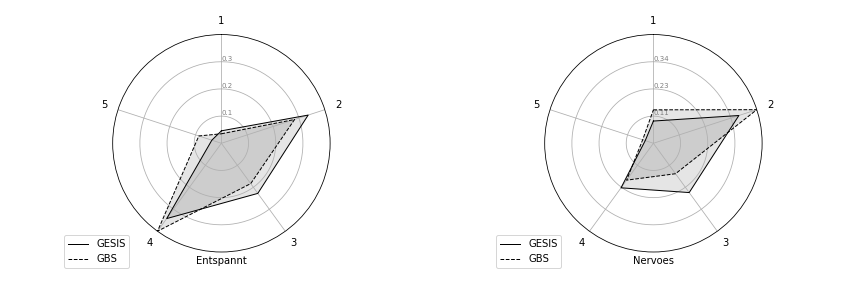
\includegraphics[scale=0.55,angle=0]{fig/Neuroticismfigure}
	         \label{Neuroticism}
	         \caption{Neuroticism: \textit{"I see myself as someone who is relaxed, handles stress well. "}(left). \textit{"I see myself as someone who gets nervous easily."}(right)..}
                \end{center}
                \end{figure}

                \begin{figure}[ht]
                \begin{center}
                   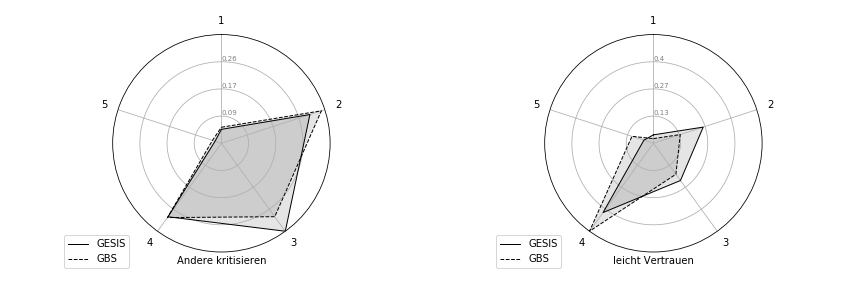
\includegraphics[scale=0.75,angle=0]{fig/Agreeablenessfigure}
	         \label{Agreeableness}
	         \caption{Agreeableness: \textit{""I see myself as someone who tends to find fault with others"}(left). \textit{"I see myself as someone who is generally trusting"}(right).}
                \end{center}
                \end{figure}

Agreeableness is the measure of one's cooperation, empathy, and willingness to trust and help others. Openness refers to openness to new experiences (i.e., whether one is timid/hesitant or eager about new objects or situations), level of inquisitiveness or curiousity, and level of preference for variety, novel stimuli and creativity. Extraversion refers to level of sociability, seeking and enjoyment of social contact, and energy and assertiveness in social situations. Extraverted people are outgoing and loquacious, while introverted people are reserved and favour solitude to social contact. Positive high affect (emotion) is linked to this concept. Neuroticism is characterized by easily experiencing disagreeable or negative emotions (anger, disappointment, frustration, etc.), and a poor coping response to those emotions

 is still ongoing debate on whether to use a Likert scale item as categorical or numeric feature. The intervals between positions on the scale are monotonic but never so well-defined as to be numerically uniform increments. A "Strongly Agree (5)" response indicates more agreement than "Agree", but it does not show agreement that is five times stronger than "Strongly Disagree (1)". 

There is an underlying measurement continuum, but  
This project treats the responses as if they fell on an interval scale.

Figure X. shows the response distribution of values for "Conscientiousness" of GBS and GESIS participants (see Appendix for a visualization of distribution shifts in "Agreeableness", "Openness", "Extraversion" and "Neuroticism").

Since GESIS and GBS analyse  on a group level should be relatively insensitive to problems that may arise.

In all these cases each aggregate measure (perhaps the mean) is based on many individual responses (e.g., n=50, 100, 1000, etc.). In these cases the original Likert item begins to take on properties that resemble an interval scale at the aggregate level.
life satisfaction of states or countries,
job satisfaction of departments,

The graphs are almost identical for the Likert item "Gruendlich". Kiviat diagrams are chosen over bar plots and histograms, as the data is not continuous but values are still related. The cyclic structure of the chart, i.e. "Strongly Disagree" next to Strongly Agree", provides a vivid example for the central-tendency bias across all items.

\subsection{Demographics and Personal Data}

\begin{table}[ht]
    \begin{center}
            {\footnotesize
            \begin{tabular}{l|c|ccccccccc}
                \hline \hline
		attribute & GBS values & GBS values count &  GBS values & GBS values count \\
                \hline \hline
                     Wach & 4 & 311 & Einigermassen & 1697 \\
                     & 3 & 183 & Erheblich & 1389 \\
                     & 2 & 66 & Ein bisschen & 467 \\ 
              	& 1 & 14 & Aeusserst & 367 \\	
		& -1 & 1 & Gar nicht & 184 \\		
		& -9 & 1 & & \\
		\hline
		Wach & 4 & 311 & Einigermassen & 1697 \\
                     & 3 & 183 & Erheblich & 1389 \\
            \end{tabular}}
        \caption{Caption.}
\end{center}
\end{table}

\section{Likert-Type Mismatch}

\begin{figure}[ht]
	\begin{center}
		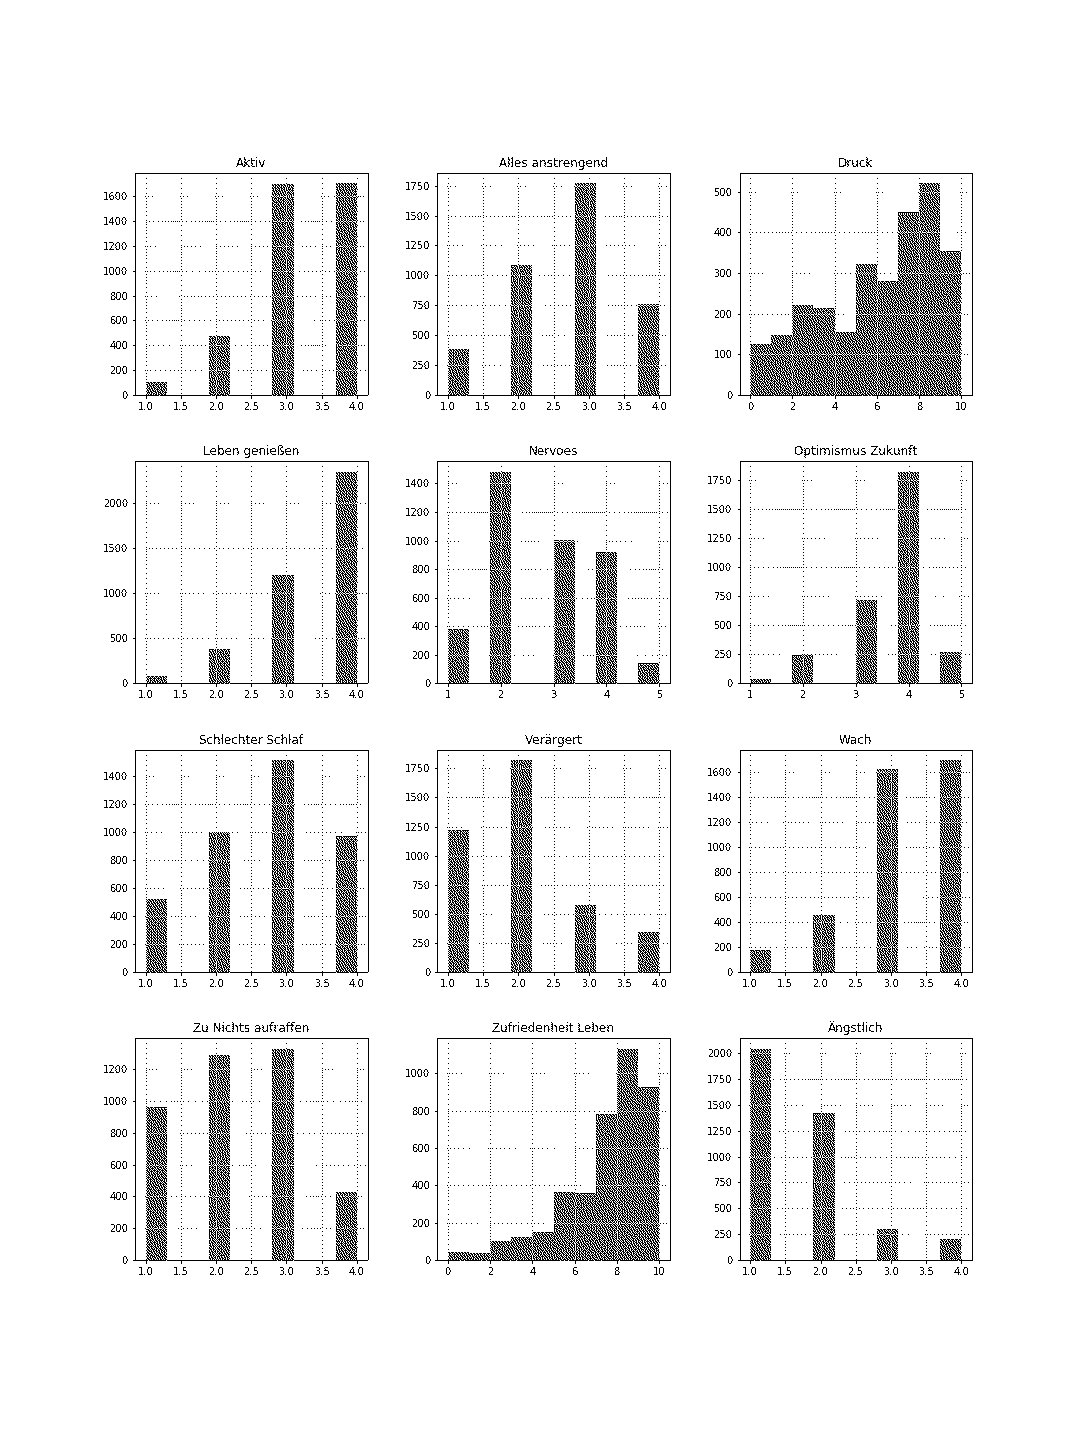
\includegraphics[scale=0.44,angle=0]{fig/gesis_hist}
		\label{std}
		\caption{GESIS hists.}
	\end{center}
\end{figure}

\begin{figure}[ht]
	\begin{center}
		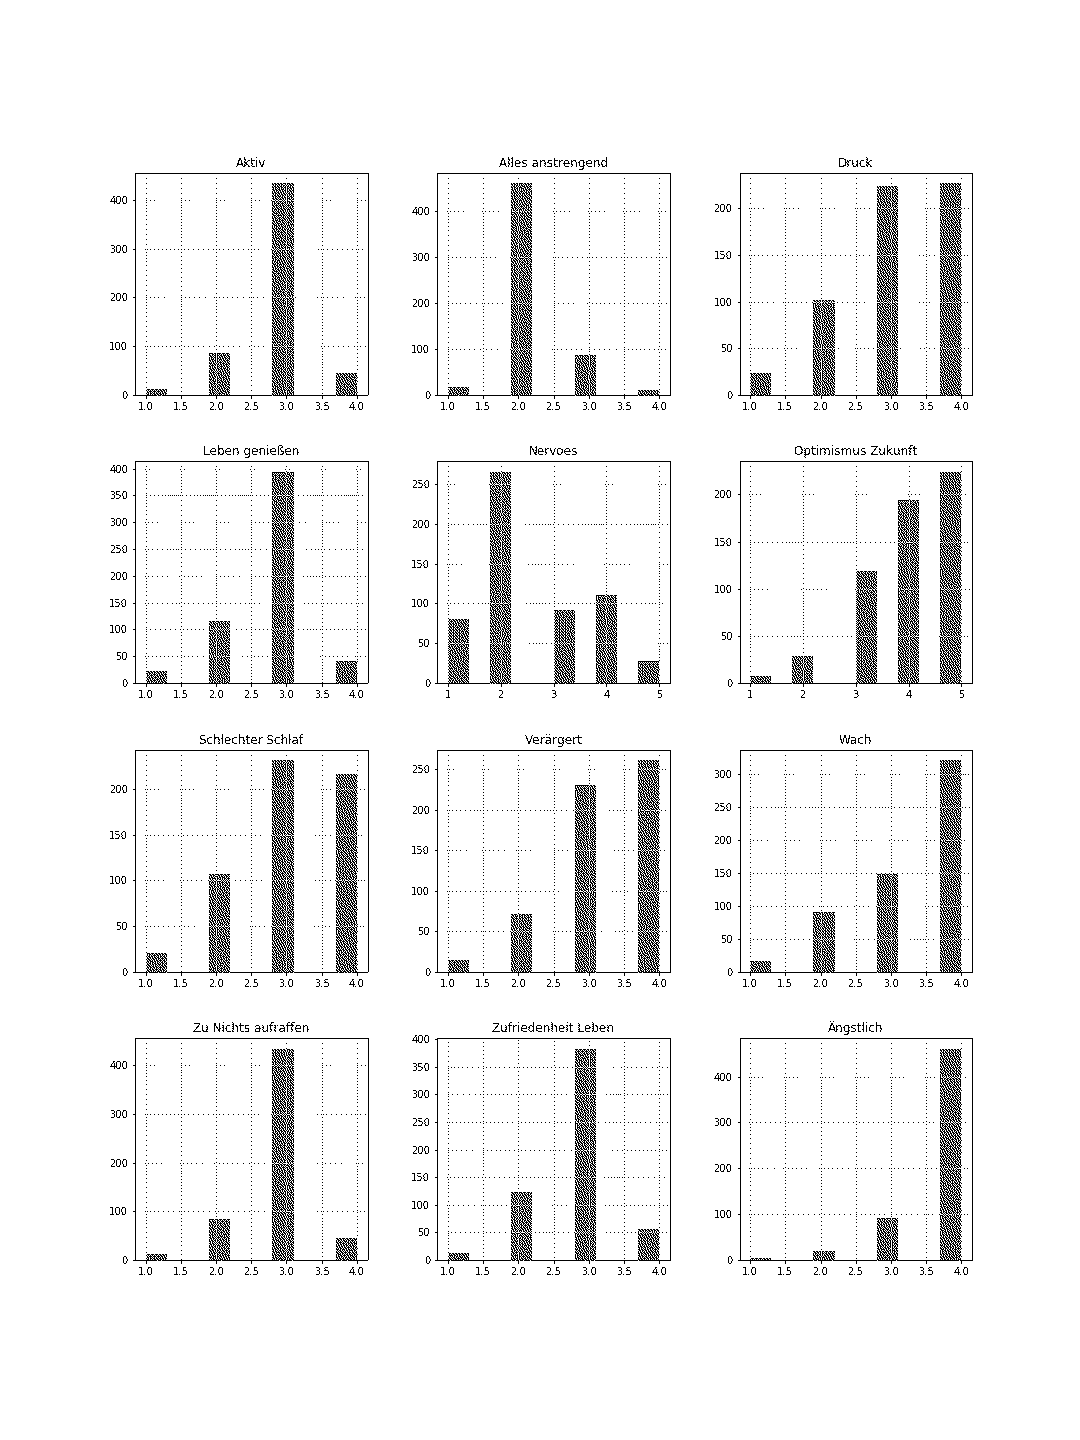
\includegraphics[scale=0.44,angle=0]{fig/gbs_hist}
		\label{std}
		\caption{GBS hists.}
	\end{center}
\end{figure}

John Tukey wrote otherwise (back in 1960) in a monograph "Data Analysis and Behavioral Science" (published in Collected Works v. III). One result he obtained is that if you're getting better than about 10percent test-retest agreement, your scale isn't narrow enough!

[1] It is confirmed that different numbers of rating bars in a subjective rating scale can have significant effects on the subjective measurement, thus the assessment of the Big Five dimensions of personality.

Techniques for reducing the length of scales while maintaining psychometric quality.
Figure X shows an example of such as a statement.

\begin{figure}[ht]
	\begin{center}
		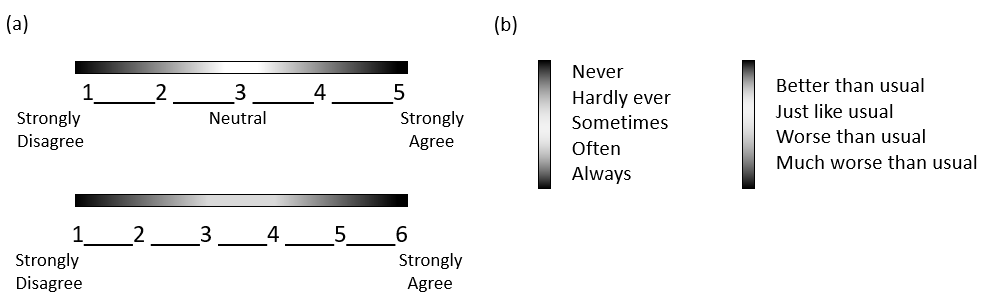
\includegraphics[scale=0.55,angle=0]{fig/scales}
		\label{6_5}
		\caption{Example of a Likert item discrepancy. GBS uses an odd number of responses with a "neutral" option, such as "no opinion", "neither agree nor disagree" or some phrase to that effect. In contrast, there is an even number of responses for this item in GESIS encouraging participants to voice a positive or negative opinion.}
	\end{center}
\end{figure}

In some cases, an additional "opt-out" option is provided for those respondents who truly cannot respond in GBS only.

\begin{table}[ht]
    \begin{center}
            {\footnotesize
            \begin{tabular}{l|c|ccccccccc}
                \hline \hline
		Raw Data & GESIS & 1 & 2 & 3 & 4 & 5 & 6 \\
                     & GBS & 1 & 2 & 3 & 4 & 5 & \\
                \hline
		Max Scaler & GESIS & 0.83 & 1.7 & 2.5 & 3.3 & 4.2 & 5.0 \\
                     & GBS & 1 & 2 & 3 & 4 & 5 & \\
                \hline
		Min-Max Scaler & GESIS & 1 & 1.8 & 2.6 & 3.4 & 4.2 & 5 \\
                     & GBS & 1.0 & 2.25 & 3.5 & 4.75 & 6.0 & \\
                \hline
		Cut-Off Mapping & GESIS & 1 & 2 & 3 & 4 & 5 & 5 \\
                     & GBS & 1 & 2 & 3 & 4 & 5 & \\
            \end{tabular}}
        \caption{Different value scalings of attribute "Desinteresse Politiker".}
\label{Tab:DescripStatsRawData}
\end{center}
\end{table}

